\documentclass{article}
\usepackage{graphicx} % Required for inserting images
\usepackage[rightcaption]{sidecap}
\usepackage[style=alphabetic]{biblatex}

\graphicspath{ {./images/} }
\addbibresource{sample.bib}

\title{Assignment 4 Report}
\author{Ole Rößler (7211)}
\date{December 2024}

\begin{document}

\maketitle
\tableofcontents

\newpage
\section{Design Exercise: Flight Booking System}

\subsection{Requirements}
This section talks about the functional and non-functional requirements of the flight booking system wanted by the ACME Organization. 
The main points given were about the given points considering (this will be a short overview about the task).

Short Description what the differences between function and non-function requirements are and I chose them (from the given context and my personal thought).

\subsubsection{Functional Requirements}
\begin{enumerate}

\item \textbf{Fetching Data:}
Periodically receive flight data updates from partner airlines (every hour).
\item \textbf{View Flights:}
The customer is able to see specific flight details. 
Therefore the customer enters a specific flight number/ flight ID and gets updates about the specified flight.
\item \textbf{Booking:}
The customer is able to book a flight on a desired flight as well as make a seat reservation on the airplane (Most airlines offer different price-tiers for seats). 
\end{enumerate}

\subsubsection{Non-Functional Requirements}
\begin{enumerate}
\item \textbf{Price Consistency:}
The system has to maintain consistency in pricing, therefore short term increases in flight-prices have to be avoided .
\item \textbf{Performance:}
Low latency for user interactions (response within seconds).
\item \textbf{Scalability:}
The system has to handle hundreds of thousands of concurrent users as well as hundreds of flights send in their data on the hour.
\item \textbf{Fault tolerance:}
The system has to be reliable.
\end{enumerate}

\subsection{System Architecture}
-> micro-services(APIs?)
-> load-balancer
-> distributed databases
-> caching to improve read performance for frequent searches
-> back up?
\begin{figure}[h]
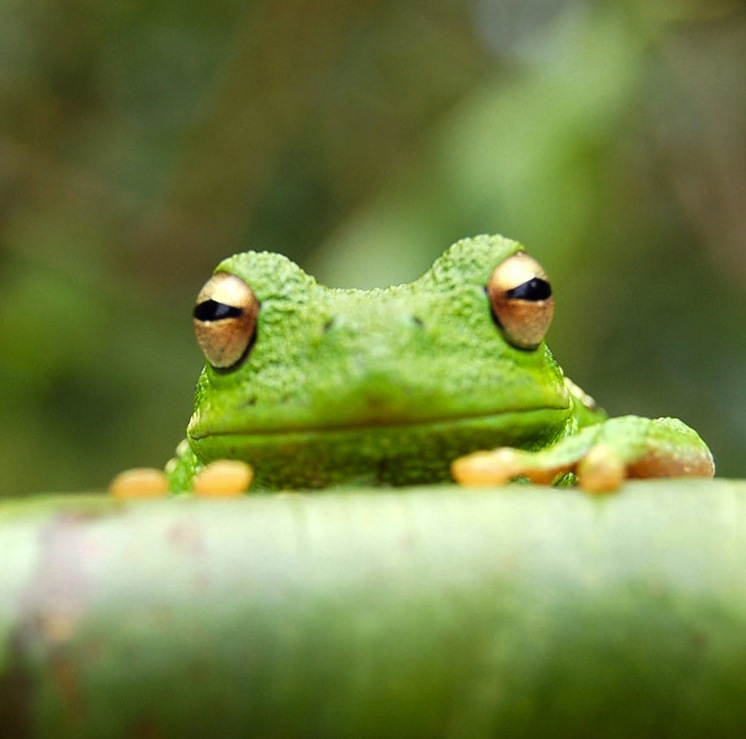
\includegraphics[width=\textwidth]{frog.jpg}
\caption{Design of my architecture}
\end{figure}






\subsection{Discussion}
TODO

\section{Freestyle Exercise}
\subsection{My DS-Concept}

\subsection{Evaluation}

\printbibliography[heading=bibintoc]
\end{document}
